\documentclass[a4paper,12pt,fleqn]{article}
\usepackage[margin=2cm]{geometry} % Definindo margens menores
\usepackage{enumitem}
\usepackage{titling}
\usepackage{lipsum} % Apenas para gerar texto de exemplo
\usepackage{listings}
\usepackage{xcolor}
\usepackage{tikz}
\usepackage{amsmath}
\usepackage{hyperref}
\usetikzlibrary{shapes, arrows, positioning}

\definecolor{codegreen}{rgb}{0,0.6,0}
\definecolor{codegray}{rgb}{0.5,0.5,0.5}
\definecolor{codepurple}{rgb}{0.58,0,0.82}
\definecolor{backcolour}{rgb}{0.95,0.95,0.92}

\lstdefinestyle{mystyle}{
    backgroundcolor=\color{backcolour},
    commentstyle=\color{codegreen},
    keywordstyle=\color{magenta},
    numberstyle=\tiny\color{codegray},
    stringstyle=\color{codepurple},
    basicstyle=\ttfamily\small,
    breakatwhitespace=false,
    breaklines=true,
    captionpos=b,
    keepspaces=true,
    numbers=left,
    numbersep=5pt,
    showspaces=false,
    showstringspaces=false,
    showtabs=false,
    tabsize=2
}

\lstset{style=mystyle}

\title{CPS769 - Introdução à Inteligência Artificial e Aprendizagem Generativa}
\author{Ellizeu Rodrigues Sena}
\date{\today}

% Definindo o cabeçalho
\renewcommand{\maketitle}{%
  \noindent\textbf{\thetitle}\\
  \textbf{Nome: \theauthor}\\
  \textbf{Professores: Edmundo de Souza e Silva}\\
  \textbf{\textcolor{white}{Professores:} Rosa M. Leão}\\
  \textbf{\textcolor{white}{Professores:} Gaspare Bruno}\\
}


\begin{document}

  \maketitle

  \section*{Lista 5}

    \subsection*{Exercício 1}
    
    O artigo escolhido foi: \textbf{Generating Text with Recurrent Neural Networks}
    
    O código utilizado para a geração de texto está disponível no GitHub: \\
    https://github.com/ellizeurs/Lista-5-CPS769
    
    \begin{figure}[h]
      \centering
      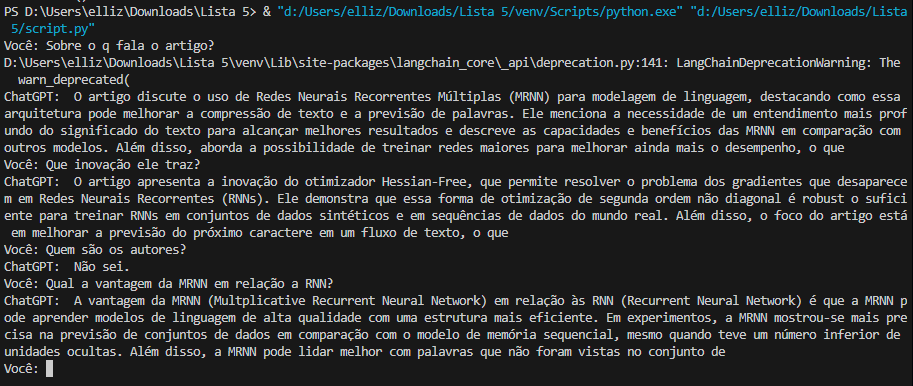
\includegraphics[width=0.8\textwidth]{assets/resposta.png}
      \caption{Resultado da geração de texto}
    \end{figure}

    Foi possível responder perguntas gerais sobre o artigo, mas perguntas como autores, data, local de publicação não foram respondidas.

    Encontrei em alguns tutoriais a inserção do texto recuperado direto no contexto, de acordo com a similaridade, mas não consegui calcular a similaridade e parece não ser feito no tutorial da LangChain.
\end{document}
